\documentclass{article}

\title{COMP101P C Coursework}
\author{Alexander Saoutkin}
\usepackage{graphicx}
\usepackage{float}
\usepackage{listings}
\usepackage[margin=1in]{geometry}
\begin{document}
\maketitle
\newpage
\section{Application Description}
I have produced a project in which a user can draw a graph in real-time by
using values from a potentiometer. 
I have chosen to allow the user to try and draw the $ sin(x) $ and $ cos(x) $
graphs. Users are given feedback in the form of the graph that is being plotted
in real-time and by LEDs indicating how close they are to the actual graphs
they are attempting to draw. In this case, a green LED means they are fairly
close to the graph, yellow means they are a bit further away and red means 
they're drawing skills are not up to scratch (and so should play a bit more).

The program is split between the arduino and an executable run on the computer.
\subsection{Arduino Code}
The arduino has two simple tasks to carry out:
\begin{enumerate}
\item Send the value of the potentiometer over the serial port to the PC/laptop.
\item Set which LED should be on based on what character the program on the 
PC/laptop sends over the serial port to the arduino.
\end{enumerate}
\subsection{PC/Laptop Code}
This program is run in conjuction with the gnuplot program. The C program
running on the PC has three main functions that it carries out as follows:
\begin{enumerate}
\item Generate the script that gnuplot will execute based on user input.
\item Calculate the next point to plot on the graph.
\item Determine which LED should light up on the Arduino.
\end{enumerate}
\subsubsection{Plotting points}
The user always starts drawing the graph on the $y$-axis. For example if the
user is attempting to draw a $sin(x)$ graph they will start drawing from (0, 0)
and if they are drawing $cos(x)$ then they will start from (0, 1). From then on
each point will be plotted with the help of polar coordinates:
\begin{figure}[H]
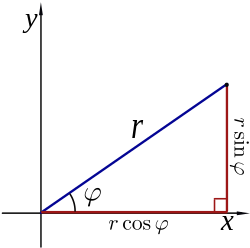
\includegraphics[height=100px]{polar}
\centering
\end{figure}
The modulus, $r$, is set at 0.05. This, in my opinion, is a good modulus for
seeing the graph being drawn in real time. The argument, $\varphi$, is determined
by the value of the potentiometer. The user can use the potentiometer to represent
arguments from $[\frac{-\pi}{2}, \frac{\pi}{2}]$. The program constantly iterates
using the previous coordinates as the center of the next point.
\section{Setting Up the Project}
\subsection{Arduino Setup}
The arduino should be setup with the breadboard as follows:
\begin{figure}[H]
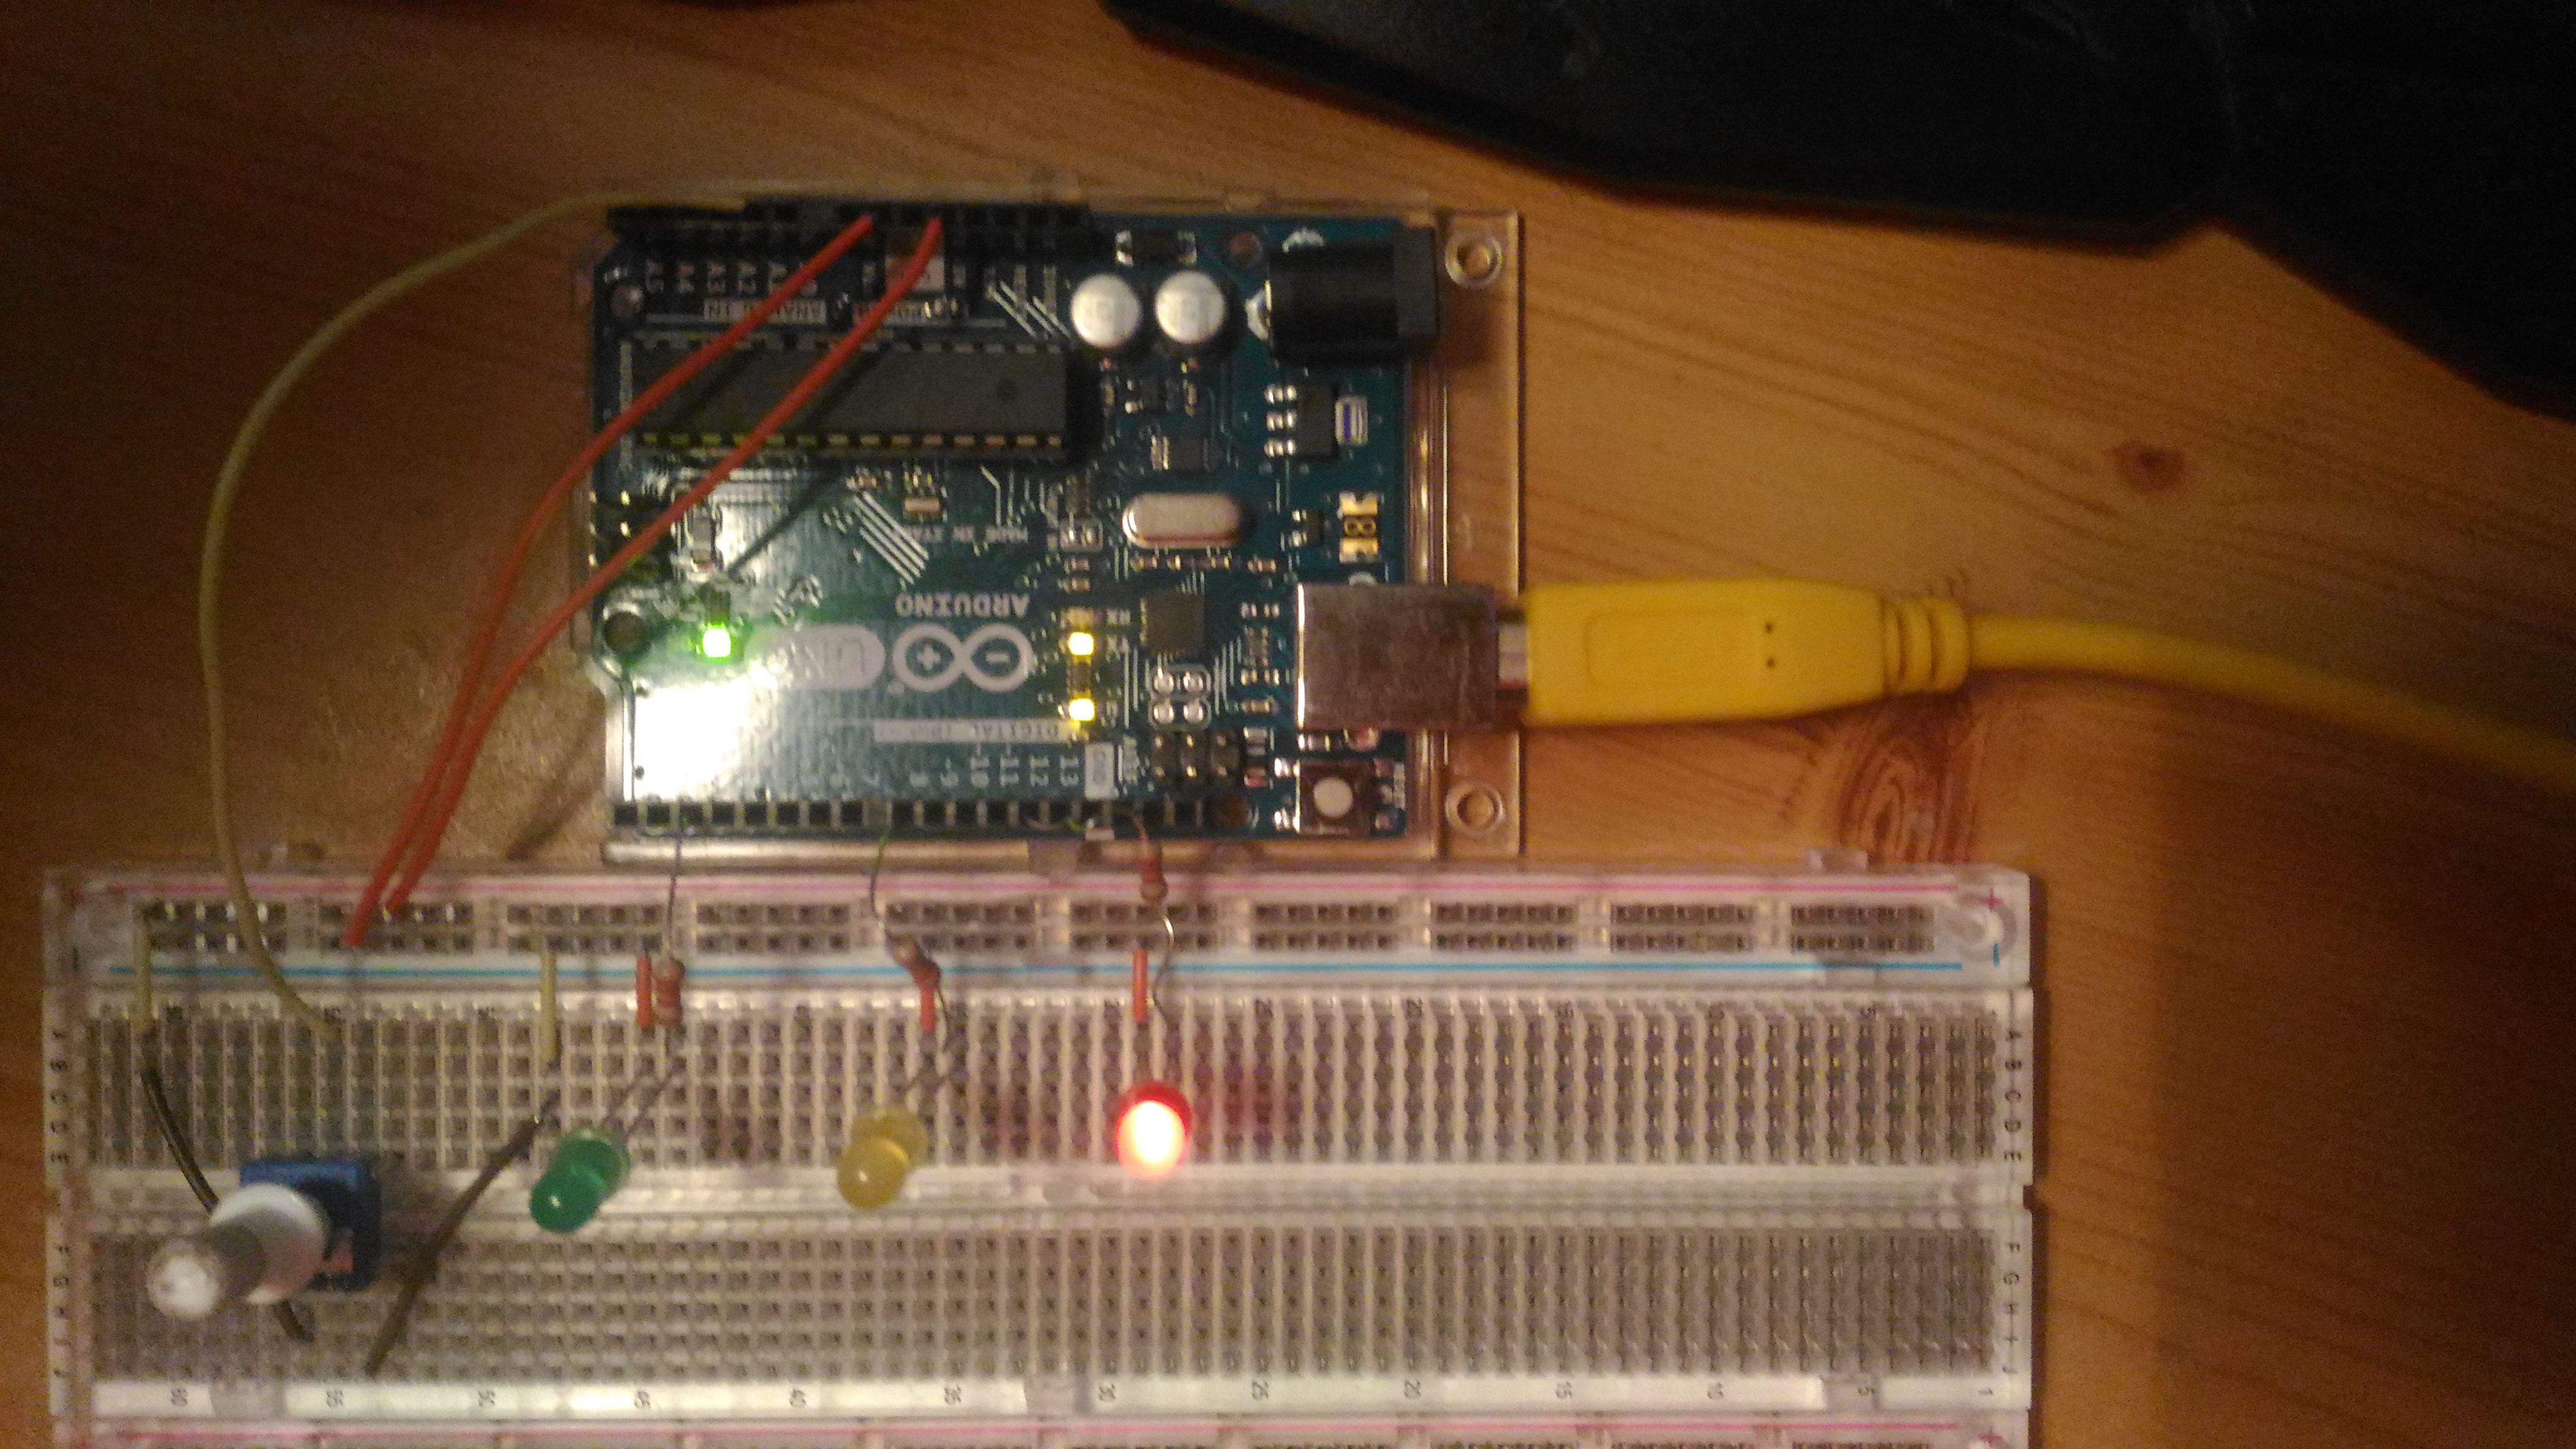
\includegraphics[width=\linewidth]{breadboard}
\end{figure}
The arduino code can be compiled by installing the platformio package and simply running the following command in the arduino code directory:
\begin{lstlisting}[language=bash]
$ sudo make upload
\end{lstlisting}
The following code can be compiled
\end{document}
